\chapter{System Kernel}\label{ch:kernel}

\section{Kernel introduction}

The RMP kernel provides the simplest functions that a usable real-time operating system must have: threads, thread delays, a mailbox mechanism, and a semaphore mechanism.
If the user needs more complex mechanisms, they can be built from these basic mechanisms.
The system also provides a lightweight graphical interface library, which consumes no memory when it is not used.\footnote{No relevant macros are defined.}

The system is recommended for applications with fewer than 32 priorities and fewer than 64 threads.
Theoretically, the number of threads and priorities is unlimited, but for efficiency and ease of use, applications beyond this complexity are not recommended.
For more complex embedded applications, a higher-level system such as RME (M7M01) is recommended.

\subsection{Kernel scheduler}

The RMP scheduler is a fully preemptive fixed-priority round-robin scheduler.
It uses round-robin scheduling among threads of the same priority and preemptive scheduling between different priorities.
Unlike some RTOSes, on some architectures the RMP scheduler never disables interrupts, which preserves real-time behaviour.
When the processor has CLZ, FFS, or similar instructions, RMP can use them to accelerate the highest-priority search.

RMP has no built-in direct support for multi-core systems.\footnote{And it never will in the future.}
Multi-core support is possible by compiling several RMP copies and running one copy on each processor as a partitioned operating system, similar to Barrelfish [1].

\subsection{Memory management and memory protection}

RMP provides a memory allocator based on the two-level segregated fit (TLSF) algorithm [2][3].
Among O(1) allocators, it has high space efficiency.
Dynamic memory allocation is not recommended in small embedded systems, so the allocator should be used as little as possible.
RMP has no true memory protection: the address spaces of threads are not isolated, so application programs must follow good programming practice.

\subsection{Application updating and application modules}

Because the system is relatively small, it does not support application updating or application modules.
A complete image built with this system should normally not exceed 128\,KiB, so the whole image can be updated.
If application modules are required, the user must implement them.

\subsection{System boot sequence}

The first thread of the RMP kernel is always \texttt{RMP\_Init}, which is in the kernel code.
The init thread performs the initial system initialisation and low-power handling, and it can never stop.
It exposes two hooks, \texttt{RMP\_Init\_Hook} and \texttt{RMP\_Init\_Idle}, which bring user code into the kernel's execution.
These two interfaces are described in Section~2.6.

\section{Thread scheduling interface}

Because the whole RMP system runs in one address space, the kernel provides only the thread abstraction.
A thread can be ready, running, suspended, or blocked, and a blocked thread can have a timeout after which it returns automatically.
The suspended state can be applied to any thread, in which case the thread is temporarily prevented from executing regardless of its other state.

\begin{figure}[htbp]
    \centering
    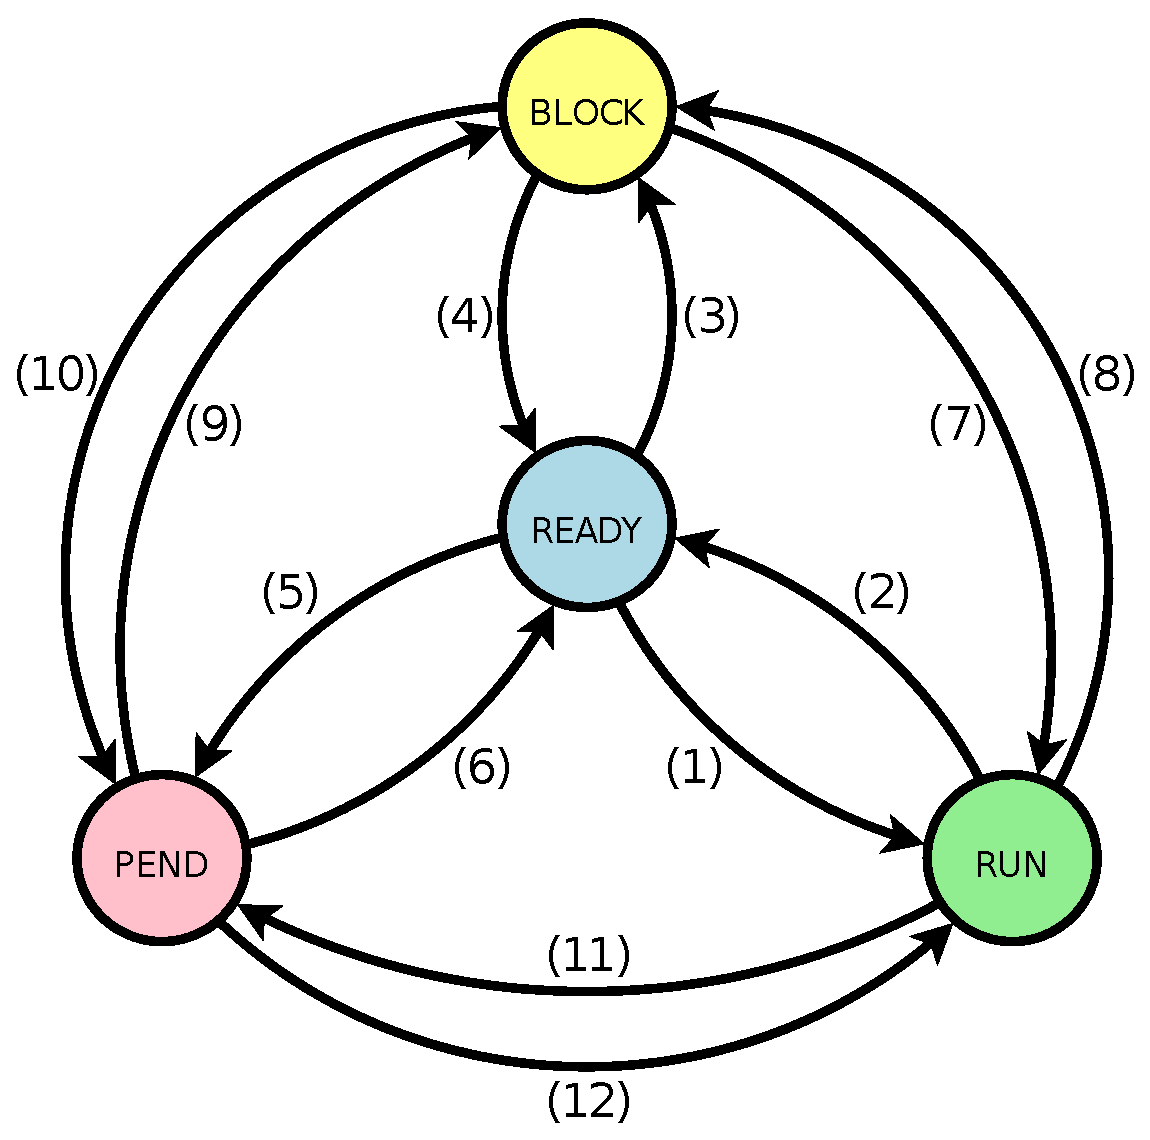
\includegraphics[width=0.72\textwidth]{Figure/thread_state.pdf}
    \caption{Thread state transition diagram.}
    \label{fig:thread-states}
\end{figure}

The numbered transitions in Figure~\ref{fig:thread-states} are explained in Table~\ref{tab:thread-transitions}.
In the figure, PEND denotes the suspended state.

\begin{table}[htbp]
    \centering
    \caption{Meaning of the transitions in Figure~\ref{fig:thread-states}.}
    \label{tab:thread-transitions}
    \small
    \begin{tabularx}{\textwidth}{@{}cX@{}}
        \toprule
        \tablehead{No.} & \tablehead{Meaning}\\
        \midrule
        (1) & The thread is ready and has the highest priority, so it moves from ready to running.\\
        (2) & The running thread is no longer the highest priority, so it moves from running to ready.\\
        (3) & This possibility does not exist; a thread cannot go directly from ready to blocked.\\
        (4) & The thread is unblocked and not suspended, and is not the highest priority, so it moves from blocked to ready.\\
        (5) & The ready thread is suspended.\\
        (6) & The suspended thread is resumed, is not blocked, and is not the highest priority, so it moves from suspended to ready.\\
        (7) & The blocked thread is unblocked, is not suspended, and is the highest priority, so it moves from blocked to running.\\
        (8) & The thread blocks on a mailbox, semaphore, or delay.\\
        (9) & The suspended thread is resumed while still blocked, so it moves from suspended to blocked.\\
        (10) & The blocked thread is suspended.\\
        (11) & The running thread is suspended.\\
        (12) & The suspended thread is resumed, is not blocked, and is the highest priority, so it moves from suspended to running.\\
        \bottomrule
    \end{tabularx}
\end{table}

The blocking state includes four basic forms: delay, waiting on a semaphore, waiting to receive from a mailbox, and waiting to send to a mailbox.\footnote{These are the four basic blocking forms in RMP.}

All thread scheduling interfaces are listed below.

\begin{apisummarytable}[H]{Thread scheduling interface summary.}{tab:thread-api}
    RMP\_Thd\_Crt     & Create a thread.
    & \cmark & \xmark \\
    RMP\_Thd\_Del     & Delete a thread. & \cmark & \xmark \\
    RMP\_Thd\_Set     & Set thread attributes. & \cmark & \xmark \\
    RMP\_Thd\_Yield   & Yield the processor. & \xmark\footnotemark & \xmark \\
    RMP\_Thd\_Suspend & Suspend a thread. & \xmark & \xmark \\
    RMP\_Thd\_Resume  & Resume a thread. & \cmark & \xmark \\
    RMP\_Thd\_Delay   & Delay a thread. & \xmark & \xmark \\
    RMP\_Thd\_Cancel  & Cancel a thread delay. & \cmark & \xmark \\
    RMP\_Thd\_Loop    & Busy-wait loop. & \cmark & \xmark \\
\end{apisummarytable}
\footnotetext{An operation that cannot block the current thread may be called
    with the scheduler locked; an operation that may block or yield the current
    thread must not.
    This criterion applies to the interfaces in later chapters as well.
}

\begin{returncodetable}[H]{Possible return values of the thread scheduling interfaces.}{tab:thread-returns}
    RMP\_ERR\_THD   & \(-1\) & Failure caused by the thread control block. \\
    RMP\_ERR\_PRIO  & \(-2\) & Failure caused by the priority. \\
    RMP\_ERR\_SLICE & \(-3\) & Failure caused by the time slice. \\
    RMP\_ERR\_STACK & \(-4\) & Failure caused by the run stack. \\
    RMP\_ERR\_STATE & \(-5\) & Failure caused by the thread state. \\
    RMP\_ERR\_OPER  & \(-6\) & Failure for any other reason. \\
\end{returncodetable}

The exact meaning of a return code in a particular function is given in that function's entry.

\subsection{Create a thread}
\begin{apidesc}{RMP\_Thd\_Crt}{Create a thread}\label{api:RMP_Thd_Crt}
    \apisig{rmp\_ret\_t RMP\_Thd\_Crt(volatile struct RMP\_Thd* Thread,
        void* Entry, void* Param, void* Stack,
        rmp\_ptr\_t Size, rmp\_ptr\_t Prio, rmp\_ptr\_t Slice)}
    This operation creates a new thread and makes it ready.
    The new thread is always inserted at the end of the time-slice round-robin queue of the same priority: if there is no other interference, the thread created first is always scheduled first.
    \begin{apiparams}
        \apiparam{volatile struct RMP\_Thd* Thread}{Pointer to an empty thread control block to be used for this thread.}
        \apiparam{void* Entry}{Entry address of the thread.}
        \apiparam{void* Param}{Parameter passed to the thread.}
        \apiparam{void* Stack}{Start address of the thread's run stack. If it is allocated as an array, fill in the first address of the array. Some architectures have special requirements for the stack memory address,\footnote{For example it must be located in the low 64\,KiB of the address space. If a stack segment register is involved, see Section~7.5.3.2.} and the address must satisfy them.}
        \apiparam{rmp\_ptr\_t Size}{Size of the thread's run stack in bytes. If it is allocated as an array, fill in the size of the array.}
        \apiparam{rmp\_ptr\_t Prio}{Priority of the thread. In this system, the larger the number, the higher the priority.}
        \apiparam{rmp\_ptr\_t Slice}{Number of time slices of the thread. The unit is clock ticks.}
    \end{apiparams}
    When \texttt{RMP\_STKSEG\_ENABLE} is non-zero, there is an additional \texttt{rmp\_ptr\_t Segment} parameter between \texttt{Param} and \texttt{Stack}, giving the thread's stack segment.
    \begin{apiret}
        \apiretval{rmp\_ret\_t}{0 on success. On failure, one of the following may be returned: \texttt{RMP\_ERR\_PRIO} if the priority is not less than \texttt{RMP\_PREEMPT\_PRIO\_NUM}; \texttt{RMP\_ERR\_SLICE} if the slice is 0 or not less than \texttt{RMP\_SLICE\_MAX}; \texttt{RMP\_ERR\_STACK} if the stack area is 0 (NULL) or too small for the context; \texttt{RMP\_ERR\_THD} if the control block is 0 (NULL) or already in use.}
    \end{apiret}
\end{apidesc}

\subsection{Delete a thread}
\begin{apidesc}{RMP\_Thd\_Del}{Delete a thread}\label{api:RMP_Thd_Del}
    \apisig{rmp\_ret\_t RMP\_Thd\_Del(volatile struct RMP\_Thd* Thread)}
    This operation deletes a thread in the system.
    After the thread is deleted, all resources are released, and the send waits of threads that are sending to it are released and return a send failure.
    Note that an RMP thread is not allowed to exit by returning.
    If any thread wants to terminate itself, it must explicitly call this function to delete itself.
    This design is intentional, to explicitly remind the user that the thread is being deleted and to help the user avoid the ``create--run once--delete'' usage as much as possible.\footnote{This usage should be replaced by ``block--run once--block again'' or thread-pool technology.}
    \begin{apiparams}
        \apiparam{volatile struct RMP\_Thd* Thread}{Pointer to the thread control block of the thread to delete.}
    \end{apiparams}
    \begin{apiret}
        \apiretval{rmp\_ret\_t}{0 on success; \texttt{RMP\_ERR\_THD} if the control block is 0 (NULL) or unused.}
    \end{apiret}
\end{apidesc}

\subsection{Set thread attributes}
\begin{apidesc}{RMP\_Thd\_Set}{Set thread attributes}\label{api:RMP_Thd_Set}
    \apisig{rmp\_ret\_t RMP\_Thd\_Set(volatile struct RMP\_Thd* Thread,
        rmp\_ptr\_t Prio, rmp\_ptr\_t Slice)}
    This operation sets the time slice and priority of a thread.
    When only one of them is to be set, simply ensure that the other parameter is \texttt{RMP\_PREEMPT\_PRIO\_NUM} or \texttt{RMP\_SLICE\_MAX}.
    \begin{apiparams}
        \apiparam{volatile struct RMP\_Thd* Thread}{Pointer to the thread control block of the thread whose priority and time slice are to be changed.}
        \apiparam{rmp\_ptr\_t Prio}{Priority to set. Entering \texttt{RMP\_PREEMPT\_PRIO\_NUM} means the priority is not changed. In this system, the larger the number, the higher the priority.}
        \apiparam{rmp\_ptr\_t Slice}{Number of time slices to set. Entering \texttt{RMP\_SLICE\_MAX} means the time slice is not changed.}
    \end{apiparams}
    \begin{apiret}
        \apiretval{rmp\_ret\_t}{0 on success. On failure: \texttt{RMP\_ERR\_PRIO} if the priority is greater than \texttt{RMP\_PREEMPT\_PRIO\_NUM}; \texttt{RMP\_ERR\_SLICE} if the slice is 0 or greater than \texttt{RMP\_SLICE\_MAX}; \texttt{RMP\_ERR\_THD} if the control block is 0 (NULL) or unused.}
    \end{apiret}
\end{apidesc}

\subsection{Yield the processor}
\begin{apidesc}{RMP\_Thd\_Yield}{Yield the processor}\label{api:RMP_Thd_Yield}
    \apisig{void RMP\_Thd\_Yield(void)}
    This operation makes the current thread give up the CPU, and the scheduler automatically selects the next thread to schedule.
    If the current thread has the highest priority and is the only thread at that priority, it is still scheduled.
    \begin{apiparams}
        \apiparam{None}{No parameters.}
    \end{apiparams}
    \begin{apiret}
        \apiretval{None}{No return value.}
    \end{apiret}
\end{apidesc}

\subsection{Suspend a thread}
\begin{apidesc}{RMP\_Thd\_Suspend}{Suspend a thread}\label{api:RMP_Thd_Suspend}
    \apisig{rmp\_ret\_t RMP\_Thd\_Suspend(volatile struct RMP\_Thd* Thread)}
    This operation suspends a thread, making the scheduler temporarily stop scheduling it.
    A thread can be suspended in any state, but its existing delay, send, receive, or other states continue to exist; that is, the suspended state is superimposed on one of the delay, send, receive, and other states.
    When the delay, send, receive, or other state ends, if the thread is still suspended, it is placed in the pure suspended state and still does not participate in scheduling until the suspended state is manually removed.
    \begin{apiparams}
        \apiparam{volatile struct RMP\_Thd* Thread}{Pointer to the thread control block of the thread to suspend.}
    \end{apiparams}
    \begin{apiret}
        \apiretval{rmp\_ret\_t}{0 on success. On failure: \texttt{RMP\_ERR\_THD} if the control block is 0 (NULL) or unused; \texttt{RMP\_ERR\_STATE} if the thread is already suspended and cannot be suspended again. This check is performed even when \texttt{RMP\_CHECK\_ENABLE} is disabled.}
    \end{apiret}
\end{apidesc}

\subsection{Resume a suspended thread}
\begin{apidesc}{RMP\_Thd\_Resume}{Resume a thread}\label{api:RMP_Thd_Resume}
    \apisig{rmp\_ret\_t RMP\_Thd\_Resume(volatile struct RMP\_Thd* Thread)}
    This operation removes a thread's suspended state, giving it a chance to participate in scheduling again.
    \begin{apiparams}
        \apiparam{volatile struct RMP\_Thd* Thread}{Pointer to the thread control block of the thread to resume.}
    \end{apiparams}
    \begin{apiret}
        \apiretval{rmp\_ret\_t}{0 on success. On failure: \texttt{RMP\_ERR\_THD} if the control block is 0 (NULL) or unused; \texttt{RMP\_ERR\_STATE} if the thread is not suspended and cannot be resumed. This check is performed even when \texttt{RMP\_CHECK\_ENABLE} is disabled.}
    \end{apiret}
\end{apidesc}

\subsection{Delay a thread}
\begin{apidesc}{RMP\_Thd\_Delay}{Delay a thread}\label{api:RMP_Thd_Delay}
    \apisig{rmp\_ret\_t RMP\_Thd\_Delay(rmp\_ptr\_t Slice)}
    This operation delays the current thread for a period of time.
    \begin{apiparams}
        \apiparam{rmp\_ptr\_t Slice}{Time to delay, in time slices.}
    \end{apiparams}
    \begin{apiret}
        \apiretval{rmp\_ret\_t}{0 on success. On failure: \texttt{RMP\_ERR\_SLICE} if the slice is 0 or not less than \texttt{RMP\_SLICE\_MAX}; \texttt{RMP\_ERR\_OPER} if the delay is cancelled before it completes. This check is performed even when \texttt{RMP\_CHECK\_ENABLE} is disabled.}
    \end{apiret}
\end{apidesc}

\subsection{Cancel a thread delay}
\begin{apidesc}{RMP\_Thd\_Cancel}{Cancel a thread delay}\label{api:RMP_Thd_Cancel}
    \apisig{rmp\_ret\_t RMP\_Thd\_Cancel(volatile struct RMP\_Thd* Thread)}
    This operation cancels a thread's delay.
    \begin{apiparams}
        \apiparam{volatile struct RMP\_Thd* Thread}{Pointer to the thread control block of the thread whose delay is to be cancelled.}
    \end{apiparams}
    \begin{apiret}
        \apiretval{rmp\_ret\_t}{0 on success. On failure: \texttt{RMP\_ERR\_THD} if the control block is 0 (NULL) or unused; \texttt{RMP\_ERR\_STATE} if the thread is not in the delay state and cannot be cancelled. This check is performed even when \texttt{RMP\_CHECK\_ENABLE} is disabled.}
    \end{apiret}
\end{apidesc}

\subsection{Thread busy-wait}
\begin{apidesc}{RMP\_Thd\_Loop}{Busy-wait a thread}\label{api:RMP_Thd_Loop}
    \apisig{void RMP\_Thd\_Loop(rmp\_ptr\_t Loop)}
    This operation makes the current thread enter a dead loop for a period of time.
    Unlike other thread interfaces, it can be used with the scheduler locked or interrupts disabled, and the delay granularity is fine, but it wastes processor performance.
    \begin{apiparams}
        \apiparam{rmp\_ptr\_t Loop}{Time to delay, in loop counts. The conversion between loop counts and processor cycles may differ with different processors, toolchains, and optimisation levels.}
    \end{apiparams}
    \begin{apiret}
        \apiretval{None}{No return value.}
    \end{apiret}
\end{apidesc}

\subsection{Peek at the next thread from an ISR}
\begin{apidesc}{RMP\_Thd\_Peek\_ISR}{Peek at the next thread from an ISR}\label{api:RMP_Thd_Peek_ISR}
    \apisig{volatile struct RMP\_Thd* RMP\_Thd\_Peek\_ISR(void)}
    This operation can be used in an interrupt or with the scheduler lock held to peek at the thread that will replace the current thread.
    If no event that can unblock a thread has occurred in the system, the thread that replaces the current thread is the thread returned by this function.
    As a special case, if the current thread is the highest-priority ready thread and there are other ready threads at that priority besides the current thread, this operation returns the next thread after the current thread, that is, the thread that would be selected if \texttt{RMP\_Thd\_Yield} were called at this moment.
    The main purpose of this operation is to periodically detect whether a high-priority thread is ready in a long critical section of a low-priority thread that uses the scheduler lock; if so, the low-priority thread can give up the scheduler lock early to reduce interrupt latency.
    \begin{apiparams}
        \apiparam{None}{No parameters.}
    \end{apiparams}
    \begin{apiret}
        \apiretval{volatile struct RMP\_Thd*}{Pointer to the control block of the next thread.}
    \end{apiret}
\end{apidesc}

\section{Thread mailbox and semaphore interface}

RMP provides simple and efficient inter-thread communication mechanisms, including thread mailboxes and semaphores.
A semaphore has an operation count, queued waiting, blocking and unlocking, and broadcast wake-up, so it can serve as a condition variable, a counter, or a lock inside a thread.
These two basic mechanisms can be used separately or combined into more complex communication interfaces.
Every blocking communication interface has three options: return immediately after detecting that blocking is possible, return after a blocking timeout, or block forever.
This greatly increases the flexibility of the interfaces.
Note that when several threads are blocked on any communication interface, they are always served in chronological order; priority jumping is not supported.
If a high-priority thread blocks after a low-priority thread, the low-priority thread is served first and the high-priority thread second.

All thread mailbox and semaphore interfaces are listed below.

\begin{apisummarytable}{Thread mailbox and semaphore interface summary.}{tab:ipc-api}
    RMP\_Thd\_Snd          & Send to a thread mailbox.
    & \xmark & \xmark \\
    RMP\_Thd\_Snd\_ISR     & Send to a thread mailbox from an interrupt. & \xmark & \cmark \\
    RMP\_Thd\_Rcv          & Receive from a thread mailbox. & \xmark & \xmark \\
    RMP\_Sem\_Crt          & Create a semaphore. & \cmark & \xmark \\
    RMP\_Sem\_Del          & Delete a semaphore. & \cmark & \xmark \\
    RMP\_Sem\_Post         & Post to a semaphore. & \cmark & \xmark \\
    RMP\_Sem\_Post\_ISR    & Post to a semaphore from an interrupt. & \xmark & \cmark \\
    RMP\_Sem\_Bcst         & Broadcast a semaphore. & \cmark & \xmark \\
    RMP\_Sem\_Bcst\_ISR    & Broadcast a semaphore from an interrupt. & \xmark & \cmark \\
    RMP\_Sem\_Pend         & Wait on a semaphore. & \xmark & \xmark \\
    RMP\_Sem\_Pend\_Unlock & Wait on a semaphore and unlock the scheduler. & \cmark\ (single lock) & \xmark \\
    RMP\_Sem\_Abort        & Abort a semaphore wait. & \cmark & \xmark \\
    RMP\_Sem\_Cnt          & Query a semaphore count. & \cmark & \xmark \\
\end{apisummarytable}

They may return the following values.

\begin{returncodetable}{Possible return values of the thread mailbox and semaphore interfaces.}{tab:ipc-returns}
    RMP\_ERR\_THD   & \(-1\) & The thread control block caused the operation to fail.
    \\
    RMP\_ERR\_SLICE & \(-3\) & The time slice caused the operation to fail. \\
    RMP\_ERR\_STATE & \(-5\) & The thread state caused the operation to fail. \\
    RMP\_ERR\_OPER  & \(-6\) & The operation failed for another reason. \\
    RMP\_ERR\_SEM   & \(-7\) & The semaphore control block caused the operation to fail. \\
\end{returncodetable}

\subsection{Send to a thread mailbox}
\begin{apidesc}{RMP\_Thd\_Snd}{Send to a thread mailbox}\label{api:RMP_Thd_Snd}
    \apisig{rmp\_ret\_t RMP\_Thd\_Snd(volatile struct RMP\_Thd* Thread,
        rmp\_ptr\_t Data, rmp\_ptr\_t Slice)}
    This operation sends a value to a thread's mailbox.
    If the mailbox is empty, the value is stored; if the receiver is waiting, it is woken.
    If the mailbox is full, the sending thread blocks.
    \begin{apiparams}
        \apiparam{volatile struct RMP\_Thd* Thread}{Pointer to the thread control block of the receiving thread.}
        \apiparam{rmp\_ptr\_t Data}{Value to send.}
        \apiparam{rmp\_ptr\_t Slice}{Number of time slices to wait if the mailbox is full. 0 means return immediately if blocking would occur; a value from 0 to \texttt{RMP\_SLICE\_MAX} means wait at most that many slices; a value greater than or equal to \texttt{RMP\_SLICE\_MAX} means wait forever.}
    \end{apiparams}
    \begin{apiret}
        \apiretval{rmp\_ret\_t}{0 on success. On failure: \texttt{RMP\_ERR\_THD} if the control block is 0 (NULL) or unused; \texttt{RMP\_ERR\_OPER} if blocking would occur with a zero timeout, if the operation is a self-send, or if the wait timed out or the target thread was deleted. The last check is performed even when \texttt{RMP\_CHECK\_ENABLE} is disabled.}
    \end{apiret}
\end{apidesc}

\subsection{Send to a thread mailbox from an interrupt}
\begin{apidesc}{RMP\_Thd\_Snd\_ISR}{Send to a thread mailbox from an ISR}\label{api:RMP_Thd_Snd_ISR}
    \apisig{rmp\_ret\_t RMP\_Thd\_Snd\_ISR(volatile struct RMP\_Thd* Thread,
        rmp\_ptr\_t Data)}
    This operation sends a value to a thread's mailbox from an interrupt vector.
    Unlike the ordinary send, it always returns immediately and does not block.
    \begin{apiparams}
        \apiparam{volatile struct RMP\_Thd* Thread}{Pointer to the thread control block of the receiving thread.}
        \apiparam{rmp\_ptr\_t Data}{Value to send.}
    \end{apiparams}
    \begin{apiret}
        \apiretval{rmp\_ret\_t}{0 on success. On failure: \texttt{RMP\_ERR\_THD} if the control block is 0 (NULL) or unused; \texttt{RMP\_ERR\_OPER} if the mailbox is full. This check is performed even when \texttt{RMP\_CHECK\_ENABLE} is disabled.}
    \end{apiret}
\end{apidesc}

\subsection{Receive from a thread mailbox}
\begin{apidesc}{RMP\_Thd\_Rcv}{Receive from a thread mailbox}\label{api:RMP_Thd_Rcv}
    \apisig{rmp\_ret\_t RMP\_Thd\_Rcv(rmp\_ptr\_t* Data, rmp\_ptr\_t Slice)}
    This operation receives a value from the current thread's mailbox.
    If the mailbox is empty, the receiving thread blocks.
    \begin{apiparams}
        \apiparam{rmp\_ptr\_t* Data}{Output pointer for the received value. If \texttt{RMP\_NULL} is passed, the received value is discarded.}
        \apiparam{rmp\_ptr\_t Slice}{Number of time slices to wait if the mailbox is empty. 0 means return immediately if blocking would occur; a value from 0 to \texttt{RMP\_SLICE\_MAX} means wait at most that many slices; a value greater than or equal to \texttt{RMP\_SLICE\_MAX} means wait forever.}
    \end{apiparams}
    \begin{apiret}
        \apiretval{rmp\_ret\_t}{0 on success. On failure: \texttt{RMP\_ERR\_OPER} if blocking would occur with a zero timeout, or if the wait timed out. This check is performed even when \texttt{RMP\_CHECK\_ENABLE} is disabled.}
    \end{apiret}
\end{apidesc}

\subsection{Create a semaphore}
\begin{apidesc}{RMP\_Sem\_Crt}{Create a semaphore}\label{api:RMP_Sem_Crt}
    \apisig{rmp\_ret\_t RMP\_Sem\_Crt(volatile struct RMP\_Sem* Semaphore,
        rmp\_ptr\_t Number)}
    This operation creates a counting semaphore.
    \begin{apiparams}
        \apiparam{volatile struct RMP\_Sem* Semaphore}{Pointer to an empty semaphore control block to be used.}
        \apiparam{rmp\_ptr\_t Number}{Initial count of the semaphore. It should be less than \texttt{RMP\_SEM\_CNT\_MAX}.}
    \end{apiparams}
    \begin{apiret}
        \apiretval{rmp\_ret\_t}{0 on success. On failure: \texttt{RMP\_ERR\_SEM} if the control block is 0 (NULL) or already used; \texttt{RMP\_ERR\_OPER} if the count is not less than \texttt{RMP\_SEM\_CNT\_MAX}.}
    \end{apiret}
\end{apidesc}

\subsection{Delete a semaphore}
\begin{apidesc}{RMP\_Sem\_Del}{Delete a semaphore}\label{api:RMP_Sem_Del}
    \apisig{rmp\_ret\_t RMP\_Sem\_Del(volatile struct RMP\_Sem* Semaphore)}
    This operation deletes a semaphore.
    If any thread is blocked on it, that thread's semaphore-wait function returns \texttt{RMP\_ERR\_OPER} directly.
    \begin{apiparams}
        \apiparam{volatile struct RMP\_Sem* Semaphore}{Pointer to the semaphore control block to delete.}
    \end{apiparams}
    \begin{apiret}
        \apiretval{rmp\_ret\_t}{0 on success; \texttt{RMP\_ERR\_SEM} if the control block is 0 (NULL) or unused.}
    \end{apiret}
\end{apidesc}

\subsection{Post to a semaphore}
\begin{apidesc}{RMP\_Sem\_Post}{Post to a semaphore}\label{api:RMP_Sem_Post}
    \apisig{rmp\_ret\_t RMP\_Sem\_Post(volatile struct RMP\_Sem* Semaphore,
        rmp\_ptr\_t Number)}
    This operation posts a number of counts to a semaphore and wakes waiting threads while the count remains positive.
    \begin{apiparams}
        \apiparam{volatile struct RMP\_Sem* Semaphore}{Pointer to the semaphore control block.}
        \apiparam{rmp\_ptr\_t Number}{Number of counts to post. It must not be 0.}
    \end{apiparams}
    \begin{apiret}
        \apiretval{rmp\_ret\_t}{0 on success. On failure: \texttt{RMP\_ERR\_SEM} if the control block is 0 (NULL) or unused; \texttt{RMP\_ERR\_OPER} if the number is 0 or the resulting count would reach \texttt{RMP\_SEM\_CNT\_MAX}.}
    \end{apiret}
\end{apidesc}

\subsection{Post to a semaphore from an interrupt}
\begin{apidesc}{RMP\_Sem\_Post\_ISR}{Post to a semaphore from an ISR}\label{api:RMP_Sem_Post_ISR}
    \apisig{rmp\_ret\_t RMP\_Sem\_Post\_ISR(volatile struct RMP\_Sem* Semaphore,
        rmp\_ptr\_t Number)}
    This operation posts a number of counts to a semaphore from an interrupt vector.
    It never blocks.
    \begin{apiparams}
        \apiparam{volatile struct RMP\_Sem* Semaphore}{Pointer to the semaphore control block.}
        \apiparam{rmp\_ptr\_t Number}{Number of counts to post. It must not be 0.}
    \end{apiparams}
    \begin{apiret}
        \apiretval{rmp\_ret\_t}{0 on success. On failure: \texttt{RMP\_ERR\_SEM} if the control block is 0 (NULL) or unused; \texttt{RMP\_ERR\_OPER} if the number is 0 or the resulting count would reach \texttt{RMP\_SEM\_CNT\_MAX}.}
    \end{apiret}
\end{apidesc}

\subsection{Broadcast a semaphore}
\begin{apidesc}{RMP\_Sem\_Bcst}{Broadcast a semaphore}\label{api:RMP_Sem_Bcst}
    \apisig{rmp\_ret\_t RMP\_Sem\_Bcst(volatile struct RMP\_Sem* Semaphore)}
    This operation wakes all threads waiting on a semaphore and returns the number of threads woken.
    The semaphore count is not changed.
    \begin{apiparams}
        \apiparam{volatile struct RMP\_Sem* Semaphore}{Pointer to the semaphore control block.}
    \end{apiparams}
    \begin{apiret}
        \apiretval{rmp\_ret\_t}{Number of threads woken on success; \texttt{RMP\_ERR\_SEM} if the control block is 0 (NULL) or unused.}
    \end{apiret}
\end{apidesc}

\subsection{Broadcast a semaphore from an interrupt}
\begin{apidesc}{RMP\_Sem\_Bcst\_ISR}{Broadcast a semaphore from an ISR}\label{api:RMP_Sem_Bcst_ISR}
    \apisig{rmp\_ret\_t RMP\_Sem\_Bcst\_ISR(volatile struct RMP\_Sem* Semaphore)}
    This operation wakes all threads waiting on a semaphore from an interrupt vector and returns the number of threads woken.
    \begin{apiparams}
        \apiparam{volatile struct RMP\_Sem* Semaphore}{Pointer to the semaphore control block.}
    \end{apiparams}
    \begin{apiret}
        \apiretval{rmp\_ret\_t}{Number of threads woken on success; \texttt{RMP\_ERR\_SEM} if the control block is 0 (NULL) or unused.}
    \end{apiret}
\end{apidesc}

\subsection{Wait on a semaphore}
\begin{apidesc}{RMP\_Sem\_Pend}{Wait on a semaphore}\label{api:RMP_Sem_Pend}
    \apisig{rmp\_ret\_t RMP\_Sem\_Pend(volatile struct RMP\_Sem* Semaphore,
        rmp\_ptr\_t Slice)}
    This operation tries to acquire a semaphore.
    If the count is positive, the count is decremented and the call returns the remaining count; otherwise the current thread blocks.
    \begin{apiparams}
        \apiparam{volatile struct RMP\_Sem* Semaphore}{Pointer to the semaphore control block.}
        \apiparam{rmp\_ptr\_t Slice}{Number of time slices to wait if the semaphore count is 0. 0 means return immediately if blocking would occur; a value from 0 to \texttt{RMP\_SLICE\_MAX} means wait at most that many slices; a value greater than or equal to \texttt{RMP\_SLICE\_MAX} means wait forever.}
    \end{apiparams}
    \begin{apiret}
        \apiretval{rmp\_ret\_t}{On success, the remaining semaphore count when the semaphore was acquired immediately, or 0 when the thread was woken after blocking. On failure: \texttt{RMP\_ERR\_SEM} if the control block is 0 (NULL) or unused; \texttt{RMP\_ERR\_OPER} if blocking would occur with a zero timeout, or if the wait timed out, was aborted, or the semaphore was deleted. This check is performed even when \texttt{RMP\_CHECK\_ENABLE} is disabled.}
    \end{apiret}
\end{apidesc}

\subsection{Wait on a semaphore and unlock the scheduler}
\begin{apidesc}{RMP\_Sem\_Pend\_Unlock}{Wait on a semaphore and unlock the scheduler}\label{api:RMP_Sem_Pend_Unlock}
    \apisig{rmp\_ret\_t RMP\_Sem\_Pend\_Unlock(volatile struct RMP\_Sem* Semaphore,
        rmp\_ptr\_t Slice)}
    This operation tries to acquire a semaphore when the scheduler is already locked; it automatically unlocks the scheduler on exit.
    \begin{apiparams}
        \apiparam{volatile struct RMP\_Sem* Semaphore}{Pointer to the semaphore control block.}
        \apiparam{rmp\_ptr\_t Slice}{Number of time slices to wait if the semaphore count is 0.}
    \end{apiparams}
    \begin{apiret}
        \apiretval{rmp\_ret\_t}{On success, the remaining count or 0 as for \texttt{RMP\_Sem\_Pend}. On failure: \texttt{RMP\_ERR\_SEM} if the control block is 0 (NULL) or unused; \texttt{RMP\_ERR\_OPER} if the scheduler lock count is not exactly one, if blocking would occur with a zero timeout, or if the wait timed out, was aborted, or the semaphore was deleted. The last two checks are performed even when \texttt{RMP\_CHECK\_ENABLE} is disabled. In the lock-count error case the function still calls \texttt{RMP\_Sched\_Unlock} once, so the caller must account for that decrement and must not unlock twice.}
    \end{apiret}
\end{apidesc}

\subsection{Abort a semaphore wait}
\begin{apidesc}{RMP\_Sem\_Abort}{Abort a semaphore wait}\label{api:RMP_Sem_Abort}
    \apisig{rmp\_ret\_t RMP\_Sem\_Abort(volatile struct RMP\_Thd* Thread)}
    This operation aborts a thread's wait for a semaphore.
    \begin{apiparams}
        \apiparam{volatile struct RMP\_Thd* Thread}{Pointer to the thread control block whose semaphore wait is to be aborted.}
    \end{apiparams}
    \begin{apiret}
        \apiretval{rmp\_ret\_t}{0 on success. On failure: \texttt{RMP\_ERR\_THD} if the control block is 0 (NULL) or unused; \texttt{RMP\_ERR\_STATE} if the thread is not waiting on a semaphore. This check is performed even when \texttt{RMP\_CHECK\_ENABLE} is disabled.}
    \end{apiret}
\end{apidesc}

\subsection{Query a semaphore count}
\begin{apidesc}{RMP\_Sem\_Cnt}{Query a semaphore count}\label{api:RMP_Sem_Cnt}
    \apisig{rmp\_ret\_t RMP\_Sem\_Cnt(volatile struct RMP\_Sem* Semaphore)}
    This operation queries the current count of a semaphore.
    \begin{apiparams}
        \apiparam{volatile struct RMP\_Sem* Semaphore}{Pointer to the semaphore control block.}
    \end{apiparams}
    \begin{apiret}
        \apiretval{rmp\_ret\_t}{Current semaphore count on success; \texttt{RMP\_ERR\_SEM} if the control block is 0 (NULL) or unused.}
    \end{apiret}
\end{apidesc}

\section{Memory management interface}

RMP provides a memory allocator based on TLSF.
It manages dynamic memory efficiently.
TLSF is a two-level fit algorithm: memory blocks are first placed into first-level intervals (FLI) by powers of two, such as 127--64 bytes and 255--128 bytes, and within each interval they are placed into linear second-level intervals (SLI).
For example, the 127--64 byte FLI has eight SLIs: [127,112], [111,96], \ldots, [79,64].
During allocation, the allocator first checks the next SLI for the requested size; if a block is available it is allocated, otherwise the nearest higher SLI is searched.
When memory is freed, the block is merged immediately and placed into the corresponding SLI for the next allocation.

In RMP's TLSF implementation, the number of FLIs is determined by the pool size and the number of SLIs is fixed at 8.
FLI 0 corresponds to 64--127 byte blocks, and a single pool must not be smaller than 1024 machine words.\footnote{For a 16-bit machine this is at least 2\,KiB; for a 32-bit machine at least 4\,KiB. Below this size there is no reason to use a pool.}
The allocator is optimised for pools below 128\,MiB and is not recommended for larger pools.
The pool and its size must both be aligned to a machine word, and the minimum allocation is 64 bytes.

The relationship between pools and threads is very flexible: one-to-one, one-to-many, many-to-one, or many-to-many.
To maximise performance in the single-thread case, the RMP memory interfaces do not provide multi-thread safety, which is very different from the other kernel interfaces.
If multi-thread safety is needed, it must be implemented with the scheduler lock or a semaphore.
Reads and writes outside an allocated region are forbidden; they can corrupt the allocator's data structures and cause exceptions.

\begin{table}[H]
    \centering
    \caption{Memory management interface summary.}
    \label{tab:memory-api}
    \small
    \begin{tabularx}{\textwidth}{@{}>{\ttfamily}p{3.6cm}>{\raggedright\arraybackslash}p{3.8cm}X@{}}
    \toprule
    \tablehead{Function} & \tablehead{Purpose} & \tablehead{Notes} \\
    \midrule
    RMP\_Mem\_Init & Initialise a memory pool. & \multirow{4}{=}{The memory management interfaces provide no thread safety. Multi-thread mutual exclusion must be provided by the application, for example with the scheduler lock or a semaphore.} \\
    RMP\_Malloc & Allocate from a memory pool. \\
    RMP\_Free & Return memory to a memory pool. \\
    RMP\_Realloc & Resize a memory block. \\
    \bottomrule
    \end{tabularx}
\end{table}

Apart from \texttt{RMP\_NULL}, the only possible return value is \texttt{RMP\_ERR\_MEM} (\(-8\)).

\subsection{Initialise a memory pool}
\begin{apidesc}{RMP\_Mem\_Init}{Initialise a memory pool}\label{api:RMP_Mem_Init}
    \apisig{rmp\_ret\_t RMP\_Mem\_Init(volatile void* Pool, rmp\_ptr\_t Size)}
    This operation initialises the pool according to the passed memory-pool size and address.
    The pool size and address must be aligned to a machine word.
    \begin{apiparams}
        \apiparam{volatile void* Pool}{Start address of the memory pool.}
        \apiparam{rmp\_ptr\_t Size}{Size of the memory pool.}
    \end{apiparams}
    \begin{apiret}
        \apiretval{rmp\_ret\_t}{0 on success; \texttt{RMP\_ERR\_MEM} if the pool is 0 (NULL), smaller than 1024 machine words, unaligned, or overflows.}
    \end{apiret}
\end{apidesc}

\subsection{Allocate from a memory pool}
\begin{apidesc}{RMP\_Malloc}{Allocate from a memory pool}\label{api:RMP_Malloc}
    \apisig{void* RMP\_Malloc(volatile void* Pool, rmp\_ptr\_t Size)}
    This operation tries to allocate memory from a memory pool.
    The minimum allocation is 64 bytes; if the requested size is smaller than that but greater than 0, 64 bytes are actually allocated; if the passed size is 0, allocation failure\footnote{This check is ignored when \texttt{RMP\_CHECK\_ENABLE} is disabled.} is returned directly.
    \begin{apiparams}
        \apiparam{volatile void* Pool}{Memory pool from which to allocate.}
        \apiparam{rmp\_ptr\_t Size}{Size of memory to allocate.}
    \end{apiparams}
    \begin{apiret}
        \apiretval{void*}{Pointer to the allocated memory; \texttt{RMP\_NULL} if no memory is available.}
    \end{apiret}
\end{apidesc}

\subsection{Return memory to a memory pool}
\begin{apidesc}{RMP\_Free}{Return memory to a memory pool}\label{api:RMP_Free}
    \apisig{void RMP\_Free(volatile void* Pool, void* Mem\_Ptr)}
    This operation returns memory to a memory pool.
    \texttt{Mem\_Ptr} must be an
    address returned by \texttt{RMP\_Malloc} that has not yet been returned, and it
    must be returned to the pool from which it was allocated;\footnote{These checks are ignored when \texttt{RMP\_CHECK\_ENABLE} is disabled.} otherwise the operation fails silently.
    If \texttt{Mem\_Ptr} is \texttt{RMP\_NULL}, nothing is done.
    \begin{apiparams}
        \apiparam{volatile void* Pool}{Memory pool to return to.}
        \apiparam{void* Mem\_Ptr}{Pointer to the memory to return.}
    \end{apiparams}
    \begin{apiret}
        \apiretval{None}{No return value.}
    \end{apiret}
\end{apidesc}

\subsection{Resize a memory block}
\begin{apidesc}{RMP\_Realloc}{Resize a memory block}\label{api:RMP_Realloc}
    \apisig{void* RMP\_Realloc(volatile void* Pool, void* Mem\_Ptr,
        rmp\_ptr\_t Size)}
    This operation tries to resize a memory block.
    \texttt{Mem\_Ptr} must be an
    address returned by \texttt{RMP\_Malloc} that has not yet been returned, and the
    passed pool must be the same as the one used when \texttt{RMP\_Malloc} was
    called.\footnote{These checks are ignored when \texttt{RMP\_CHECK\_ENABLE} is disabled.}
    On success, it returns the original block or a new block whose first \texttt{Size} bytes have the same contents as the original address; when \texttt{Size} is greater than 0 and less than 64, 64 bytes are allocated by default.
    On failure it returns 0 (NULL) and the original block is unaffected.
    If \texttt{Size} is 0, the behaviour is the same as \texttt{RMP\_Free} and the block is released directly.\footnote{This may differ from some implementations.}
    If \texttt{Mem\_Ptr} is \texttt{RMP\_NULL}, the behaviour is the same as \texttt{RMP\_Malloc}.
    \begin{apiparams}
        \apiparam{volatile void* Pool}{Memory pool.}
        \apiparam{void* Mem\_Ptr}{Memory block to resize.}
        \apiparam{rmp\_ptr\_t Size}{New size.}
    \end{apiparams}
    \begin{apiret}
        \apiretval{void*}{Pointer to the resized block; \texttt{RMP\_NULL} on failure or when \texttt{Size} is 0.}
    \end{apiret}
\end{apidesc}

\section{Hook function interface}

To make it convenient to insert user-required functions at some key points in system operation, RMP also provides hook functions.
Hook functions are divided into mandatory hooks and optional hooks: the former are declared as functions and must be provided; the latter are declared as macros and need not be filled in.

\subsection{Mandatory hook interface}

The hook functions that must be implemented by the user are as follows.

\subsubsection{Idle-thread first-run hook}

This hook function is called once when the idle thread first runs.
Its typical use is to create other threads, semaphores, and message queues, or to perform some system initialisation work.
Note that this hook executes with interrupts disabled throughout, so it must not call any operation that may depend on interrupts or any operation that enables interrupts.
If such operations are needed, perform them in another thread.

\begin{apidesc}{RMP\_Init\_Hook}{Idle-thread first-run hook}\label{api:RMP_Init_Hook}
    \apisig{void RMP\_Init\_Hook(void)}
    Called once when the idle thread first runs.
    \begin{apiparams}
        \apiparam{None}{No parameters.}
    \end{apiparams}
    \begin{apiret}
        \apiretval{None}{No return value.}
    \end{apiret}
\end{apidesc}

\subsubsection{Idle-thread repeated-run hook}

This hook function is called repeatedly when the idle thread runs.
Its typical use is to enter a low-power mode to save energy, or to perform performance analysis and stack-check printing.
The idle thread must not be put into a blocking state in this hook; otherwise the system will crash.

\begin{apidesc}{RMP\_Init\_Idle}{Idle-thread repeated-run hook}\label{api:RMP_Init_Idle}
    \apisig{void RMP\_Init\_Idle(void)}
    Called repeatedly when the idle thread runs.
    \begin{apiparams}
        \apiparam{None}{No parameters.}
    \end{apiparams}
    \begin{apiret}
        \apiretval{None}{No return value.}
    \end{apiret}
\end{apidesc}

\subsection{Optional hook interface}

The optional hook macros that the user may choose to implement when needed are as follows.

\subsubsection{System start hook}

If this hook macro is defined, it is called immediately after the system completes processor initialisation.
Because each port initialises only part of the most basic hardware at system startup, further hardware initialisation is recommended to be placed inside this hook.
If the desired basic system configuration conflicts with the basic initialisation provided by the platform's configuration header,\footnote{For example, configuring the system to a completely different operating frequency.} the basic system configuration can also be redone inside this hook.

\begin{apidesc}{RMP\_START\_HOOK}{System start hook}\label{api:RMP_START_HOOK}
    \apisig{void RMP\_START\_HOOK(void)}
    Called immediately after processor initialisation.
    \begin{apiparams}
        \apiparam{None}{No parameters.}
    \end{apiparams}
    \begin{apiret}
        \apiretval{None}{No return value.}
    \end{apiret}
\end{apidesc}

\subsubsection{System context-save hook}

If this hook macro is defined, it is called after the system completes basic context saving.
If additional context\footnote{FPU and other peripheral register banks.} must be saved, it can be pushed onto the stack in this function.
See Chapter~4 for the implementation method.

\begin{apidesc}{RMP\_CTX\_SAVE}{System context-save hook}\label{api:RMP_CTX_SAVE}
    \apisig{void RMP\_CTX\_SAVE(void)}
    Called after basic context saving.
    \begin{apiparams}
        \apiparam{None}{No parameters.}
    \end{apiparams}
    \begin{apiret}
        \apiretval{None}{No return value.}
    \end{apiret}
\end{apidesc}

\subsubsection{System context-restore hook}

If this hook macro is defined, it is called before the system completes basic context restoration.
If additional context\footnote{FPU and other peripheral register banks.} must be restored, it can be popped from the stack in this function.
See Chapter~4 for the implementation method.

\begin{apidesc}{RMP\_CTX\_LOAD}{System context-restore hook}\label{api:RMP_CTX_LOAD}
    \apisig{void RMP\_CTX\_LOAD(void)}
    Called before basic context restoration.
    \begin{apiparams}
        \apiparam{None}{No parameters.}
    \end{apiparams}
    \begin{apiret}
        \apiretval{None}{No return value.}
    \end{apiret}
\end{apidesc}

\subsubsection{Scheduler hook}

If this hook macro is defined, it is called when the system completes selection of the current thread.
If a tickless kernel is to be implemented, the relevant functions can be called in this hook.
See Section~7.1.1 for the implementation of a tickless system.

\begin{apidesc}{RMP\_SCHED\_HOOK}{Scheduler hook}\label{api:RMP_SCHED_HOOK}
    \apisig{void RMP\_SCHED\_HOOK(void)}
    Called after the current thread is selected.
    \begin{apiparams}
        \apiparam{None}{No parameters.}
    \end{apiparams}
    \begin{apiret}
        \apiretval{None}{No return value.}
    \end{apiret}
\end{apidesc}

\subsubsection{System tick hook}

If this hook macro is defined, it is called when the system tick arrives.

\begin{apidesc}{RMP\_TIM\_HOOK}{System tick hook}\label{api:RMP_TIM_HOOK}
    \apisig{void RMP\_TIM\_HOOK(rmp\_ptr\_t Slice)}
    Called when the system tick arrives.
    \begin{apiparams}
        \apiparam{rmp\_ptr\_t Slice}{The \texttt{Slice} parameter that \texttt{\_RMP\_Tim\_Handler} receives when called.}
    \end{apiparams}
    \begin{apiret}
        \apiretval{None}{No return value.}
    \end{apiret}
\end{apidesc}

\subsubsection{Delay-insertion hook}

If this hook macro is defined, it is called when a thread is inserted into the delay queue.

\begin{apidesc}{RMP\_DLY\_HOOK}{Delay-insertion hook}\label{api:RMP_DLY_HOOK}
    \apisig{void RMP\_DLY\_HOOK(rmp\_ptr\_t Slice)}
    Called when a thread is inserted into the delay queue.
    \begin{apiparams}
        \apiparam{rmp\_ptr\_t Slice}{The \texttt{Slice} parameter that the delayed system function receives when called.}
    \end{apiparams}
    \begin{apiret}
        \apiretval{None}{No return value.}
    \end{apiret}
\end{apidesc}

\subsubsection{Error-logging hook}

If this hook macro is defined, it is called when the system prints error information.
If it is not defined, the system prints errors to the console by default.

\begin{apidesc}{RMP\_LOG}{Error-logging hook}\label{api:RMP_Log}
    \apisig{void RMP\_LOG(const char* File, long Line, const char* Date,
        const char* Time)}
    Called when the system prints error information.
    \begin{apiparams}
        \apiparam{const char* File}{Name of the file where the error occurred.}
        \apiparam{long Line}{Line number where the error occurred.}
        \apiparam{const char* Date}{Compilation date.}
        \apiparam{const char* Time}{Compilation time.}
    \end{apiparams}
    \begin{apiret}
        \apiretval{None}{No return value.}
    \end{apiret}
\end{apidesc}

\section{Auxiliary system interface}

The other auxiliary interfaces provided by RMP include interrupt enable/disable and scheduler lock/unlock.
These interfaces provide convenience when the user writes an application.

\subsection{Interrupt and scheduler interface}

In RMP, the interrupt-system interface consists only of a pair of functions that disable and enable interrupts.
This pair is provided to the user because on some architectures RMP itself does not disable interrupts during operation.
Unless absolutely necessary, disabling interrupts is not recommended, because it greatly affects the system's real-time performance.

The scheduler-system interface consists of a pair of functions that enable and disable the scheduler with a nesting count.
This pair is also provided to the user.
Because locking the scheduler also reduces real-time performance, frequent use is not recommended.
The general policy is: if the problem can be solved without locking the scheduler, do not lock it; if both locking the scheduler and disabling interrupts can solve it, lock the scheduler; only when interrupts must be disabled should they be disabled, and the interrupt-disabled interval should be as short as possible.

\subsubsection{Disable interrupts}

This operation disables the processor's response to all interrupt sources, including the system timer interrupt and the scheduling interrupt.
This function has no nesting count; if nesting is required, the user must implement it.

\begin{apidesc}{RMP\_Int\_Disable}{Disable interrupts}\label{api:RMP_Int_Disable_Ch2}
    \apisig{void RMP\_Int\_Disable(void)}
    Disables the processor's response to all interrupt sources.
    \begin{apiparams}
        \apiparam{None}{No parameters.}
    \end{apiparams}
    \begin{apiret}
        \apiretval{None}{No return value.}
    \end{apiret}
\end{apidesc}

\subsubsection{Enable interrupts}

This operation enables the processor's response to all interrupt sources.
This function has no nesting count; if nesting is required, the user must implement it.

\begin{apidesc}{RMP\_Int\_Enable}{Enable interrupts}\label{api:RMP_Int_Enable_Ch2}
    \apisig{void RMP\_Int\_Enable(void)}
    Enables the processor's response to all interrupt sources.
    \begin{apiparams}
        \apiparam{None}{No parameters.}
    \end{apiparams}
    \begin{apiret}
        \apiretval{None}{No return value.}
    \end{apiret}
\end{apidesc}

\subsubsection{Lock the scheduler}

This operation locks the scheduler, preventing it from selecting a new thread to schedule.
This function has a nesting count.

\begin{apidesc}{RMP\_Sched\_Lock}{Lock the scheduler}\label{api:RMP_Sched_Lock}
    \apisig{void RMP\_Sched\_Lock(void)}
    Locks the scheduler.
    \begin{apiparams}
        \apiparam{None}{No parameters.}
    \end{apiparams}
    \begin{apiret}
        \apiretval{None}{No return value.}
    \end{apiret}
\end{apidesc}

\subsubsection{Unlock the scheduler}

This operation unlocks the scheduler, allowing it to select a new thread to schedule again.
This function has a nesting count.

\begin{apidesc}{RMP\_Sched\_Unlock}{Unlock the scheduler}\label{api:RMP_Sched_Unlock}
    \apisig{void RMP\_Sched\_Unlock(void)}
    Unlocks the scheduler.
    \begin{apiparams}
        \apiparam{None}{No parameters.}
    \end{apiparams}
    \begin{apiret}
        \apiretval{None}{No return value.}
    \end{apiret}
\end{apidesc}

\subsection{Auxiliary library function interface}

To make application writing convenient, RMP provides a series of library functions, including memory clearing, debug printing, and linked-list operations.
They are listed below.
The default logging function is \texttt{RMP\_Log}, and the kernel coverage printer is \texttt{RMP\_Cov\_Print}.

\subsubsection{Clear memory}

This operation clears a block of memory to zero.

\begin{apidesc}{RMP\_Clear}{Clear memory}\label{api:RMP_Clear}
    \apisig{void RMP\_Clear(volatile void* Addr, rmp\_ptr\_t Size)}
    Clears a block of memory to zero.
    \begin{apiparams}
        \apiparam{volatile void* Addr}{Start address of the memory block to clear.}
        \apiparam{rmp\_ptr\_t Size}{Size of the memory block to clear, in bytes.}
    \end{apiparams}
    \begin{apiret}
        \apiretval{None}{No return value.}
    \end{apiret}
\end{apidesc}

\subsubsection{Print one character}

This operation prints one character to the console.\footnote{Usually a serial port.}

\begin{apidesc}{RMP\_Putchar}{Print one character}\label{api:RMP_Putchar}
    \apisig{void RMP\_Putchar(char Char)}
    Prints one character to the console.
    \begin{apiparams}
        \apiparam{char Char}{The character to print.}
    \end{apiparams}
    \begin{apiret}
        \apiretval{None}{No return value.}
    \end{apiret}
\end{apidesc}

\subsubsection{Print a signed integer}

This operation prints a signed integer of one machine word in signed decimal to the debug console.

\begin{apidesc}{RMP\_Int\_Print}{Print a signed integer}\label{api:RMP_Int_Print}
    \apisig{rmp\_cnt\_t RMP\_Int\_Print(rmp\_cnt\_t Int)}
    Prints a signed integer in signed decimal.
    \begin{apiparams}
        \apiparam{rmp\_cnt\_t Int}{The signed integer to print.}
    \end{apiparams}
    \begin{apiret}
        \apiretval{rmp\_cnt\_t}{The number of characters printed.}
    \end{apiret}
\end{apidesc}

\subsubsection{Print an unsigned integer}

This operation prints an unsigned integer of one machine word in hexadecimal without a prefix to the debug console.

\begin{apidesc}{RMP\_Hex\_Print}{Print an unsigned integer}\label{api:RMP_Hex_Print}
    \apisig{rmp\_cnt\_t RMP\_Hex\_Print(rmp\_ptr\_t Uint)}
    Prints an unsigned integer in hexadecimal without a prefix.
    \begin{apiparams}
        \apiparam{rmp\_ptr\_t Uint}{The unsigned integer to print.}
    \end{apiparams}
    \begin{apiret}
        \apiretval{rmp\_cnt\_t}{The number of characters printed.}
    \end{apiret}
\end{apidesc}

\subsubsection{Print a string}

This operation prints a string of at most 255 characters to the debug console.

\begin{apidesc}{RMP\_Str\_Print}{Print a string}\label{api:RMP_Str_Print}
    \apisig{rmp\_cnt\_t RMP\_Str\_Print(const rmp\_s8\_t* String)}
    Prints a string to the debug console.
    \begin{apiparams}
        \apiparam{const rmp\_s8\_t* String}{The string to print.}
    \end{apiparams}
    \begin{apiret}
        \apiretval{rmp\_cnt\_t}{The number of characters printed.}
    \end{apiret}
\end{apidesc}

\subsubsection{Get the most significant bit of a word}

This operation obtains the bit number of the most significant bit of a word.\footnote{For example a 32-bit processor returns 0--31.}
If the number is 0, it must return $-1$.\footnote{For example a 32-bit processor should return \texttt{0xFFFFFFFF}.}
This is a generic function and cannot use processor-specific acceleration instructions; if possible, use the \texttt{RMP\_MSB\_GET} macro.

\begin{apidesc}{RMP\_MSB\_Generic}{Get the most significant bit of a word}\label{api:RMP_MSB_Generic}
    \apisig{rmp\_ptr\_t RMP\_MSB\_Generic(rmp\_ptr\_t Value)}
    Obtains the bit number of the most significant bit of a word.
    \begin{apiparams}
        \apiparam{rmp\_ptr\_t Value}{The unsigned integer whose most-significant-bit number is to be found.}
    \end{apiparams}
    \begin{apiret}
        \apiretval{rmp\_ptr\_t}{The bit number of the word's most significant bit.}
    \end{apiret}
\end{apidesc}

\subsubsection{Get the least significant bit of a word}

This operation obtains the bit number of the least significant bit of a word.\footnote{For example a 32-bit processor returns 0--31.}
If the number is 0, it returns a value equal to the processor word length.\footnote{For example a 32-bit processor returns 32.}
This is a generic function and cannot use processor-specific acceleration instructions; if possible, use the \texttt{RMP\_LSB\_GET} macro.

\begin{apidesc}{RMP\_LSB\_Generic}{Get the least significant bit of a word}\label{api:RMP_LSB_Generic}
    \apisig{rmp\_ptr\_t RMP\_LSB\_Generic(rmp\_ptr\_t Value)}
    Obtains the bit number of the least significant bit of a word.
    \begin{apiparams}
        \apiparam{rmp\_ptr\_t Value}{The unsigned integer whose least-significant-bit number is to be found.}
    \end{apiparams}
    \begin{apiret}
        \apiretval{rmp\_ptr\_t}{The bit number of the word's least significant bit.}
    \end{apiret}
\end{apidesc}

\subsubsection{Create a doubly linked circular list}

This operation initialises the head of a doubly linked circular list.

\begin{apidesc}{RMP\_List\_Crt}{Create a doubly linked circular list}\label{api:RMP_List_Crt}
    \apisig{void RMP\_List\_Crt(volatile struct RMP\_List* Head)}
    Initialises the head of a doubly linked circular list.
    \begin{apiparams}
        \apiparam{volatile struct RMP\_List* Head}{Pointer to the list-head structure to initialise.}
    \end{apiparams}
    \begin{apiret}
        \apiretval{None}{No return value.}
    \end{apiret}
\end{apidesc}

\subsubsection{Delete nodes from a doubly linked circular list}

This operation deletes one or a series of nodes from a doubly linked list.

\begin{apidesc}{RMP\_List\_Del}{Delete nodes from a doubly linked circular list}\label{api:RMP_List_Del}
    \apisig{void RMP\_List\_Del(volatile struct RMP\_List* Prev,
        volatile struct RMP\_List* Next)}
    Deletes one or a series of nodes from a doubly linked circular list.
    \begin{apiparams}
        \apiparam{volatile struct RMP\_List* Prev}{Pointer to the predecessor of the node (or node group) to delete.}
        \apiparam{volatile struct RMP\_List* Next}{Pointer to the successor of the node (or node group) to delete.}
    \end{apiparams}
    \begin{apiret}
        \apiretval{None}{No return value.}
    \end{apiret}
\end{apidesc}

\subsubsection{Insert a node into a doubly linked circular list}

This operation inserts one node into a doubly linked list.

\begin{apidesc}{RMP\_List\_Ins}{Insert a node into a doubly linked circular list}\label{api:RMP_List_Ins}
    \apisig{void RMP\_List\_Ins(volatile struct RMP\_List* New,
        volatile struct RMP\_List* Prev, volatile struct RMP\_List* Next)}
    Inserts one node into a doubly linked circular list.
    \begin{apiparams}
        \apiparam{volatile struct RMP\_List* New}{Pointer to the new node to insert.}
        \apiparam{volatile struct RMP\_List* Prev}{Pointer to the predecessor of the insertion position.}
        \apiparam{volatile struct RMP\_List* Next}{Pointer to the successor of the insertion position.}
    \end{apiparams}
    \begin{apiret}
        \apiretval{None}{No return value.}
    \end{apiret}
\end{apidesc}

\section{Chapter bibliography}

None.
